\chapter{Introduction}
\label{introduction}


The Internet of Things (\textbf{\gls{iot}}) is an interconnected network that extends Internet support and services to control and interact with smart devices, sensors, home appliances, vehicles, factory machines, wearable devices, and so on, with minimal human interaction \cite{touqeer2021smart}. \autoref{iotenvironment} shows the typical connections and services that it is possible to achieve an \gls{iot} environment.

    \begin{figure}[H]
        \centering
        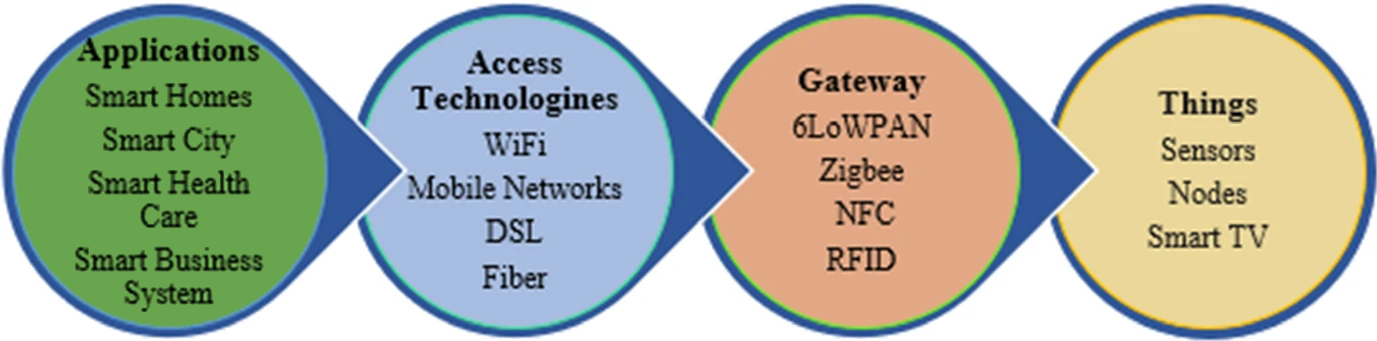
\includegraphics[scale=0.30]{images/introduction/iot_schema.jpg}
        \caption{Typical IoT Environment}
        \label{iotenvironment}
    \end{figure}

Moreover, \gls{iot} is the basis for Smart Homes. A possible definition of a \textbf{Smart Home} describes it as an \gls{iot} environment where heterogeneous electronic devices and appliances are networked together to provide services ubiquitously to individuals \cite{shouran2019internet}. Hence, a Smart Home can provide innovative and smart services to the user and improve its quality of life, and it is a consequence of the increasing growth in \gls{iot} technology \cite{kumar2017security,vimal2015internet}.

Typical Smart Home devices are smoke sensors, light bulbs, plugs, doors, thermostats, etc. In this regard, it is interesting to think about how the number of connected devices increases day by day due to miniaturization, growth, and power availability, and this trend is predicted to lead to around 500 billion devices connected to the Internet by the year 2030 with a global mobile traffic estimation of 4394 EB/month \cite{yastrebova2018future}. \autoref{globaltrend} shows the graphical representation of the described trends.

    \begin{figure}[H]
        \centering
        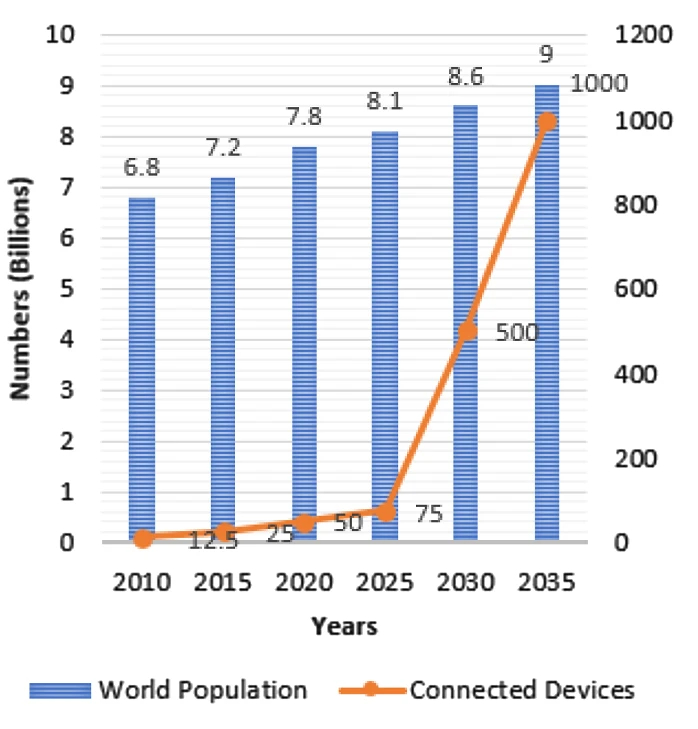
\includegraphics[scale=0.25]{images/introduction/devices_human.jpg}
        \caption{Estimated connected devices per world population \cite{touqeer2021smart}}
        \label{globaltrend}
    \end{figure}

Although Smart Homes have increased users' convenience, they are also valuable for attackers. In fact, \gls{iot}-enabled home appliances and Smart Home Gateways can be vulnerable to cyberattacks and create a point of entry to the Smart Home \cite{ray2020iot}.


The proposed work focuses on the vulnerabilities that may arise in those Smart Homes where the control center is a Smart Home Gateway that is also \textbf{extensible} by means of \textbf{add-ons} (also known as \textit{plug-ins} or \textit{integrations}). Add-ons provide additional functionalities to the Smart Home components, a representation of which may be the one in \autoref{shcomponents}.

\begin{figure}[H]
    \centering
    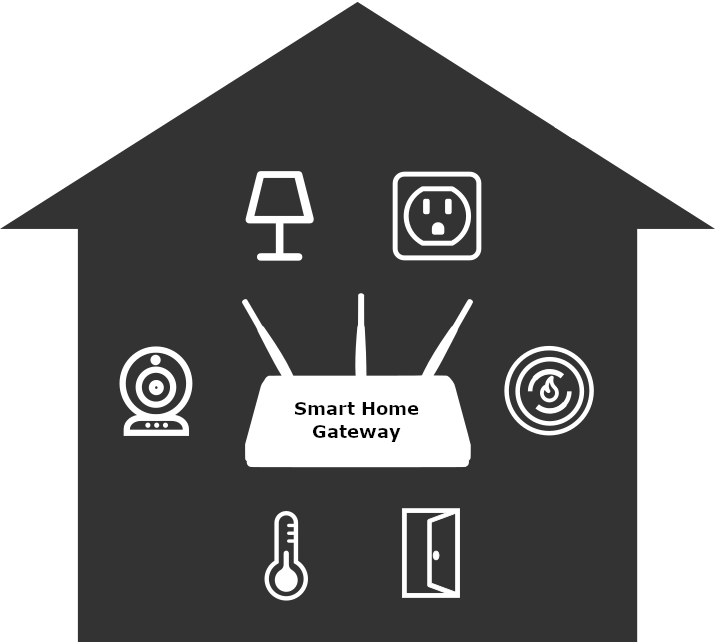
\includegraphics[scale=0.60]{images/introduction/shg_arch.png}
    \caption{Smart Home components \cite{wtabout}}
    \label{shcomponents}
\end{figure}

Starting from a threat model as a reference, the objective of this work is to understand whether add-ons developed by amateur or distracted programmers can cause some vulnerability in the Smart Home. The extensible Smart Home Gateway that will be the target of evaluation is the one provided by WebThings, an open source platform that was incubated at Mozilla for four years before being spun out as an independent open source project \cite{francismozilla, wtabout}.

Going further, the following chapters will present in \autoref{background} a brief background about Smart Home Gateways (focusing on the one provided by WebThings) and Threat Modeling. Then, in \autoref{pocs}, there will be a deep dive into the threat model used as a reference for the work and the related Proofs of Concept (\textbf{\glspl{poc}}) that have been developed to confirm the validity of the threat model guidelines. Afterwards, \autoref{experiments} will discuss the making of two different surveys having the objective to validate the \glspl{poc}. Lastly, \autoref{conclusions} will discuss the outcome of the surveys and what could be the possible future work.